\documentclass[10pt,letterpaper]{article}

\usepackage[margin=0.75in]{geometry}
\usepackage{tikz}

\begin{document}

  \title{CS 321, Assignment 1}
  \author{Cody Malick\\
  \texttt{malickc@oregonstate.edu}}
  \date{\today}
  \maketitle

\section{}

\begin{center}
	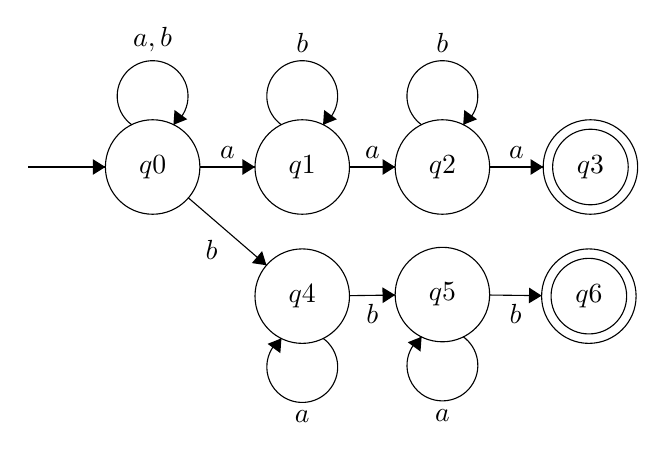
\begin{tikzpicture}[scale=0.2]
		\tikzstyle{every node}+=[inner sep=0pt]
		\draw [black] (13.9,-21.2) circle (3);
		\draw (13.9,-21.2) node {$q0$};
		\draw [black] (23.4,-21.2) circle (3);
		\draw (23.4,-21.2) node {$q1$};
		\draw [black] (32.3,-21.2) circle (3);
		\draw (32.3,-21.2) node {$q2$};
		\draw [black] (41.7,-21.2) circle (3);
		\draw (41.7,-21.2) node {$q3$};
		\draw [black] (41.7,-21.2) circle (2.4);
		\draw [black] (23.4,-29.4) circle (3);
		\draw (23.4,-29.4) node {$q4$};
		\draw [black] (32.3,-29.3) circle (3);
		\draw (32.3,-29.3) node {$q5$};
		\draw [black] (41.6,-29.4) circle (3);
		\draw (41.6,-29.4) node {$q6$};
		\draw [black] (41.6,-29.4) circle (2.4);
		\draw [black] (6,-21.2) -- (10.9,-21.2);
		\fill [black] (10.9,-21.2) -- (10.1,-20.7) -- (10.1,-21.7);
		\draw [black] (16.9,-21.2) -- (20.4,-21.2);
		\fill [black] (20.4,-21.2) -- (19.6,-20.7) -- (19.6,-21.7);
		\draw (18.65,-20.7) node [above] {$a$};
		\draw [black] (26.4,-21.2) -- (29.3,-21.2);
		\fill [black] (29.3,-21.2) -- (28.5,-20.7) -- (28.5,-21.7);
		\draw (27.85,-20.7) node [above] {$a$};
		\draw [black] (35.3,-21.2) -- (38.7,-21.2);
		\fill [black] (38.7,-21.2) -- (37.9,-20.7) -- (37.9,-21.7);
		\draw (37,-20.7) node [above] {$a$};
		\draw [black] (12.577,-18.52) arc (234:-54:2.25);
		\draw (13.9,-13.95) node [above] {$a,b$};
		\fill [black] (15.22,-18.52) -- (16.1,-18.17) -- (15.29,-17.58);
		\draw [black] (22.077,-18.52) arc (234:-54:2.25);
		\draw (23.4,-13.95) node [above] {$b$};
		\fill [black] (24.72,-18.52) -- (25.6,-18.17) -- (24.79,-17.58);
		\draw [black] (30.977,-18.52) arc (234:-54:2.25);
		\draw (32.3,-13.95) node [above] {$b$};
		\fill [black] (33.62,-18.52) -- (34.5,-18.17) -- (33.69,-17.58);
		\draw [black] (16.17,-23.16) -- (21.13,-27.44);
		\fill [black] (21.13,-27.44) -- (20.85,-26.54) -- (20.2,-27.3);
		\draw (17.64,-25.79) node [below] {$b$};
		\draw [black] (26.4,-29.37) -- (29.3,-29.33);
		\fill [black] (29.3,-29.33) -- (28.49,-28.84) -- (28.51,-29.84);
		\draw (27.85,-29.86) node [below] {$b$};
		\draw [black] (35.3,-29.33) -- (38.6,-29.37);
		\fill [black] (38.6,-29.37) -- (37.81,-28.86) -- (37.79,-29.86);
		\draw (36.95,-29.86) node [below] {$b$};
		\draw [black] (24.723,-32.08) arc (54:-234:2.25);
		\draw (23.4,-36.65) node [below] {$a$};
		\fill [black] (22.08,-32.08) -- (21.2,-32.43) -- (22.01,-33.02);
		\draw [black] (33.623,-31.98) arc (54:-234:2.25);
		\draw (32.3,-36.55) node [below] {$a$};
		\fill [black] (30.98,-31.98) -- (30.1,-32.33) -- (30.91,-32.92);
	\end{tikzpicture}
\end{center}

\section{}

\begin{center}
	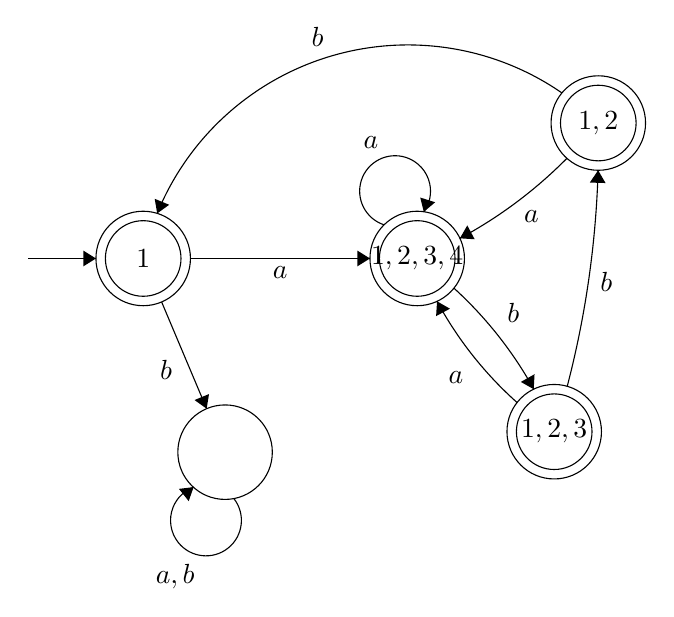
\begin{tikzpicture}[scale=0.2]
		\tikzstyle{every node}+=[inner sep=0pt]
		\draw [black] (24.5,-25.8) circle (3);
		\draw (24.5,-25.8) node {${1}$};
		\draw [black] (24.5,-25.8) circle (2.4);
		\draw [black] (29.7,-38.1) circle (3);
		\draw (29.7,-38.1) node {${}$};
		\draw [black] (41.9,-25.8) circle (3);
		\draw (41.9,-25.8) node {${1,2,3,4}$};
		\draw [black] (41.9,-25.8) circle (2.4);
		\draw [black] (50.6,-36.8) circle (3);
		\draw (50.6,-36.8) node {${1,2,3}$};
		\draw [black] (50.6,-36.8) circle (2.4);
		\draw [black] (53.4,-17.2) circle (3);
		\draw (53.4,-17.2) node {${1,2}$};
		\draw [black] (53.4,-17.2) circle (2.4);
		\draw [black] (17.2,-25.8) -- (21.5,-25.8);
		\fill [black] (21.5,-25.8) -- (20.7,-25.3) -- (20.7,-26.3);
		\draw [black] (25.67,-28.56) -- (28.53,-35.34);
		\fill [black] (28.53,-35.34) -- (28.68,-34.41) -- (27.76,-34.79);
		\draw (26.36,-32.89) node [left] {$b$};
		\draw [black] (30.251,-41.037) arc (38.35775:-249.64225:2.25);
		\draw (26.53,-45.2) node [below] {$a,b$};
		\fill [black] (27.7,-40.32) -- (26.77,-40.43) -- (27.39,-41.21);
		\draw [black] (27.5,-25.8) -- (38.9,-25.8);
		\fill [black] (38.9,-25.8) -- (38.1,-25.3) -- (38.1,-26.3);
		\draw (33.2,-26.3) node [below] {$a$};
		\draw [black] (39.807,-23.667) arc (252.1782:-35.8218:2.25);
		\draw (38.96,-18.85) node [above] {$a$};
		\fill [black] (42.32,-22.84) -- (43.04,-22.23) -- (42.09,-21.93);
		\draw [black] (44.232,-27.685) arc (47.6485:29.03308:25.273);
		\fill [black] (49.3,-34.1) -- (49.35,-33.15) -- (48.48,-33.64);
		\draw (47.59,-29.27) node [right] {$b$};
		\draw [black] (48.242,-34.948) arc (-131.74932:-151.5691:23.808);
		\fill [black] (43.16,-28.52) -- (43.1,-29.46) -- (43.98,-28.99);
		\draw (44.86,-33.37) node [left] {$a$};
		\draw [black] (53.387,-20.2) arc (-1.64564:-14.61456:61.347);
		\fill [black] (53.39,-20.2) -- (52.86,-20.98) -- (53.86,-21.01);
		\draw (53.49,-27.28) node [right] {$b$};
		\draw [black] (51.406,-19.44) arc (-44.67996:-61.73984:28.599);
		\fill [black] (44.61,-24.52) -- (45.55,-24.58) -- (45.08,-23.7);
		\draw (49.15,-22.73) node [below] {$a$};
		\draw [black] (25.387,-22.938) arc (157.77964:55.36404:17.205);
		\fill [black] (25.39,-22.94) -- (26.15,-22.39) -- (25.23,-22.01);
		\draw (35.58,-12.4) node [above] {$b$};
	\end{tikzpicture}
\end{center}


\section{}
\begin{center}
	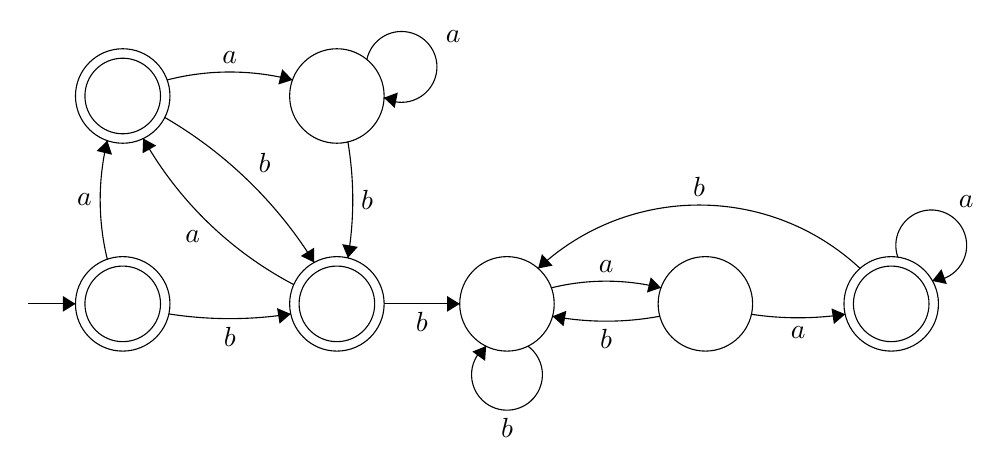
\begin{tikzpicture}[scale=0.2]
		\tikzstyle{every node}+=[inner sep=0pt]
		\draw [black] (13.8,-32.9) circle (3);
		\draw [black] (13.8,-32.9) circle (2.4);
		\draw [black] (13.8,-19.7) circle (3);
		\draw [black] (13.8,-19.7) circle (2.4);
		\draw [black] (27.4,-19.7) circle (3);
		\draw [black] (27.4,-32.9) circle (3);
		\draw [black] (27.4,-32.9) circle (2.4);
		\draw [black] (38.2,-32.9) circle (3);
		\draw [black] (50.8,-32.9) circle (3);
		\draw [black] (62.6,-32.9) circle (3);
		\draw [black] (62.6,-32.9) circle (2.4);
		\draw [black] (7.8,-32.9) -- (10.8,-32.9);
		\fill [black] (10.8,-32.9) -- (10,-32.4) -- (10,-33.4);
		\draw [black] (24.47,-33.538) arc (-81.13606:-98.86394:25.118);
		\fill [black] (24.47,-33.54) -- (23.6,-33.17) -- (23.76,-34.16);
		\draw (20.6,-34.34) node [below] {$b$};
		\draw [black] (12.821,-30.069) arc (-166.31549:-193.68451:15.931);
		\fill [black] (12.82,-22.53) -- (12.15,-23.19) -- (13.12,-23.43);
		\draw (11.87,-26.3) node [left] {$a$};
		\draw [black] (16.617,-18.682) arc (104.47348:75.52652:15.935);
		\fill [black] (24.58,-18.68) -- (23.93,-18) -- (23.68,-18.97);
		\draw (20.6,-17.68) node [above] {$a$};
		\draw [black] (28.099,-22.615) arc (9.59464:-9.59464:22.108);
		\fill [black] (28.1,-29.98) -- (28.73,-29.28) -- (27.74,-29.11);
		\draw (28.91,-26.3) node [right] {$b$};
		\draw [black] (29.301,-17.394) arc (168.22775:-119.77225:2.25);
		\draw (34.28,-15.93) node [right] {$a$};
		\fill [black] (30.39,-19.81) -- (31.07,-20.46) -- (31.27,-19.48);
		\draw [black] (16.471,-21.062) arc (59.83855:31.87165:27.358);
		\fill [black] (25.96,-30.27) -- (25.96,-29.33) -- (25.11,-29.86);
		\draw (22.8,-24.6) node [above] {$b$};
		\draw [black] (24.662,-31.678) arc (-117.7075:-150.5823:23.539);
		\fill [black] (15.1,-22.4) -- (15.06,-23.34) -- (15.93,-22.85);
		\draw (18.25,-28.21) node [below] {$a$};
		\draw [black] (30.4,-32.9) -- (35.2,-32.9);
		\fill [black] (35.2,-32.9) -- (34.4,-32.4) -- (34.4,-33.4);
		\draw (32.8,-33.4) node [below] {$b$};
		\draw [black] (39.523,-35.58) arc (54:-234:2.25);
		\draw (38.2,-40.15) node [below] {$b$};
		\fill [black] (36.88,-35.58) -- (36,-35.93) -- (36.81,-36.52);
		\draw [black] (41.017,-31.883) arc (103.91284:76.08716:14.486);
		\fill [black] (47.98,-31.88) -- (47.33,-31.21) -- (47.09,-32.18);
		\draw (44.5,-30.96) node [above] {$a$};
		\draw [black] (47.908,-33.685) arc (-79.4337:-100.5663:18.585);
		\fill [black] (41.09,-33.69) -- (41.79,-34.32) -- (41.97,-33.34);
		\draw (44.5,-34.5) node [below] {$b$};
		\draw [black] (59.677,-33.563) arc (-81.48938:-98.51062:20.116);
		\fill [black] (59.68,-33.56) -- (58.81,-33.19) -- (58.96,-34.18);
		\draw (56.7,-34.28) node [below] {$a$};
		\draw [black] (63.023,-29.942) arc (199.5918:-88.4082:2.25);
		\draw (67.36,-26.83) node [above] {$a$};
		\fill [black] (65.21,-31.44) -- (66.13,-31.64) -- (65.79,-30.7);
		\draw [black] (40.176,-30.649) arc (132.98694:47.01306:14.995);
		\fill [black] (40.18,-30.65) -- (41.1,-30.47) -- (40.42,-29.74);
		\draw (50.4,-26.12) node [above] {$b$};
	\end{tikzpicture}
\end{center}

\section{}
We know that $w\in{0,1}^* $ is a regular language. To show that it is still a
regular language given a randomly insterted substring, $011$, resulting in a
value that is a multiple of three, we simply have to show that there is a DFA
or NFA that accepts. This can be done with an NFA that starts with a modulus
three set of states, then, after the insertion of the substring, checking to
see if the resulting string is mod three.

In the following case, the transition function, $p --> 011 --> q$ is showing
that the substring $011$ has been read in. 

\begin{center}
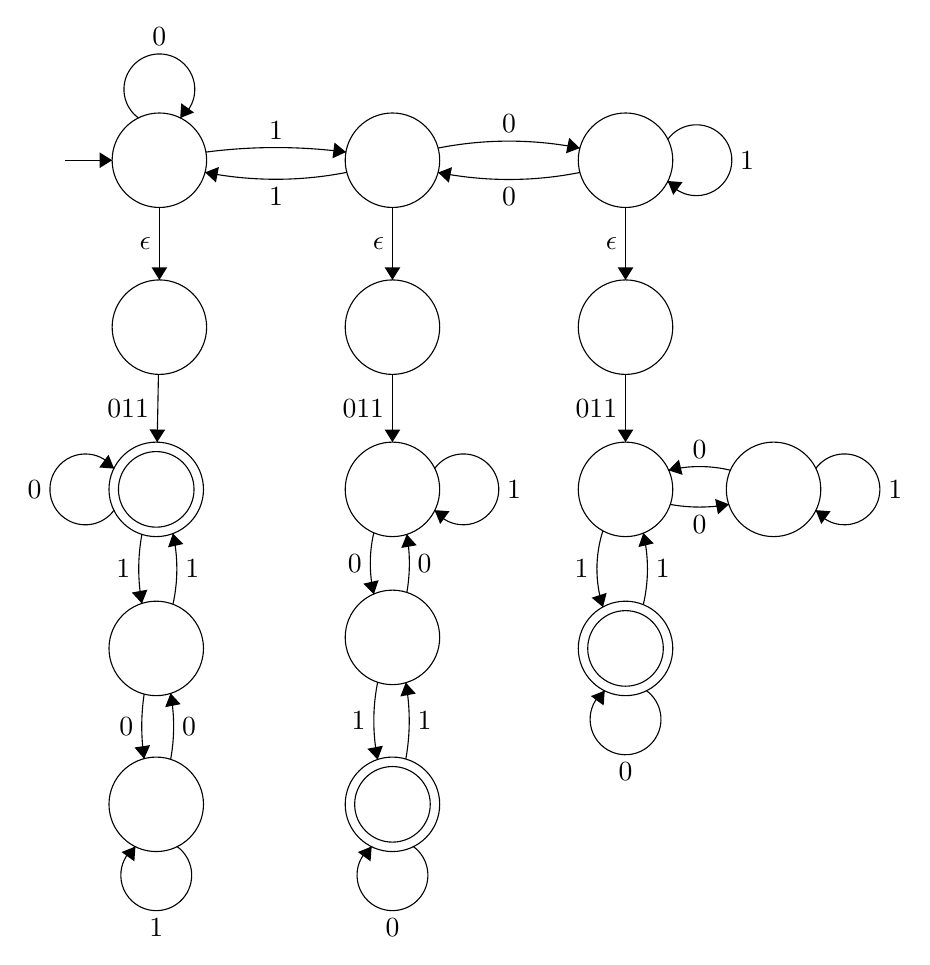
\begin{tikzpicture}[scale=0.2]
	\tikzstyle{every node}+=[inner sep=0pt]
	\draw [black] (14.5,-9.3) circle (3);
	\draw [black] (29.3,-9.3) circle (3);
	\draw [black] (44.1,-9.3) circle (3);
	\draw [black] (14.5,-19.9) circle (3);
	\draw [black] (29.3,-19.9) circle (3);
	\draw [black] (44.1,-19.9) circle (3);
	\draw [black] (14.3,-30.2) circle (3);
	\draw [black] (14.3,-30.2) circle (2.4);
	\draw [black] (14.3,-40.3) circle (3);
	\draw [black] (14.3,-50.2) circle (3);
	\draw [black] (29.3,-30.2) circle (3);
	\draw [black] (29.3,-39.6) circle (3);
	\draw [black] (29.3,-50.2) circle (3);
	\draw [black] (29.3,-50.2) circle (2.4);
	\draw [black] (44.1,-30.2) circle (3);
	\draw [black] (53.5,-30.2) circle (3);
	\draw [black] (44.1,-40.3) circle (3);
	\draw [black] (44.1,-40.3) circle (2.4);
	\draw [black] (8.5,-9.3) -- (11.5,-9.3);
	\fill [black] (11.5,-9.3) -- (10.7,-8.8) -- (10.7,-9.8);
	\draw [black] (17.454,-8.783) arc (97.42616:82.57384:34.398);
	\fill [black] (26.35,-8.78) -- (25.62,-8.18) -- (25.49,-9.18);
	\draw (21.9,-7.99) node [above] {$1$};
	\draw [black] (26.402,-10.069) arc (-78.82789:-101.17211:23.238);
	\fill [black] (17.4,-10.07) -- (18.09,-10.71) -- (18.28,-9.73);
	\draw (21.9,-11.01) node [below] {$1$};
	\draw [black] (32.197,-8.528) arc (101.21312:78.78688:23.158);
	\fill [black] (41.2,-8.53) -- (40.52,-7.88) -- (40.32,-8.86);
	\draw (36.7,-7.59) node [above] {$0$};
	\draw [black] (41.205,-10.077) arc (-78.70796:-101.29204:23.005);
	\fill [black] (32.2,-10.08) -- (32.88,-10.72) -- (33.08,-9.74);
	\draw (36.7,-11.02) node [below] {$0$};
	\draw [black] (46.78,-7.977) arc (144:-144:2.25);
	\draw (51.35,-9.3) node [right] {$1$};
	\fill [black] (46.78,-10.62) -- (47.13,-11.5) -- (47.72,-10.69);
	\draw [black] (44.1,-12.3) -- (44.1,-16.9);
	\fill [black] (44.1,-16.9) -- (44.6,-16.1) -- (43.6,-16.1);
	\draw (43.6,-14.6) node [left] {$\epsilon$};
	\draw [black] (29.3,-12.3) -- (29.3,-16.9);
	\fill [black] (29.3,-16.9) -- (29.8,-16.1) -- (28.8,-16.1);
	\draw (28.8,-14.6) node [left] {$\epsilon$};
	\draw [black] (14.5,-12.3) -- (14.5,-16.9);
	\fill [black] (14.5,-16.9) -- (15,-16.1) -- (14,-16.1);
	\draw (14,-14.6) node [left] {$\epsilon$};
	\draw [black] (13.391,-37.449) arc (-169.46661:-190.53339:12.029);
	\fill [black] (13.39,-37.45) -- (13.74,-36.57) -- (12.75,-36.75);
	\draw (12.69,-35.25) node [left] {$1$};
	\draw [black] (15.361,-32.995) arc (12.5181:-12.5181:10.403);
	\fill [black] (15.36,-33) -- (15.05,-33.88) -- (16.02,-33.67);
	\draw (16.11,-35.25) node [right] {$1$};
	\draw [black] (13.534,-47.306) arc (-171.419:-188.581:13.776);
	\fill [black] (13.53,-47.31) -- (13.91,-46.44) -- (12.92,-46.59);
	\draw (12.88,-45.25) node [left] {$0$};
	\draw [black] (15.214,-43.148) arc (10.40966:-10.40966:11.631);
	\fill [black] (15.21,-43.15) -- (14.87,-44.03) -- (15.85,-43.84);
	\draw (15.91,-45.25) node [right] {$0$};
	\draw [black] (14.44,-22.9) -- (14.36,-27.2);
	\fill [black] (14.36,-27.2) -- (14.87,-26.41) -- (13.87,-26.39);
	\draw (13.87,-25.05) node [left] {$011$};
	\draw [black] (29.3,-22.9) -- (29.3,-27.2);
	\fill [black] (29.3,-27.2) -- (29.8,-26.4) -- (28.8,-26.4);
	\draw (28.8,-25.05) node [left] {$011$};
	\draw [black] (28.12,-36.858) arc (-166.76268:-193.23732:8.553);
	\fill [black] (28.12,-36.86) -- (28.42,-35.97) -- (27.45,-36.19);
	\draw (27.39,-34.9) node [left] {$0$};
	\draw [black] (30.214,-33.047) arc (9.85026:-9.85026:10.829);
	\fill [black] (30.21,-33.05) -- (29.86,-33.92) -- (30.84,-33.75);
	\draw (30.87,-34.9) node [right] {$0$};
	\draw [black] (28.361,-47.358) arc (-168.61386:-191.38614:12.453);
	\fill [black] (28.36,-47.36) -- (28.69,-46.48) -- (27.71,-46.67);
	\draw (27.62,-44.9) node [left] {$1$};
	\draw [black] (30.149,-42.471) arc (10.2004:-10.2004:13.715);
	\fill [black] (30.15,-42.47) -- (29.8,-43.35) -- (30.78,-43.17);
	\draw (30.87,-44.9) node [right] {$1$};
	\draw [black] (15.623,-52.88) arc (54:-234:2.25);
	\draw (14.3,-57.45) node [below] {$1$};
	\fill [black] (12.98,-52.88) -- (12.1,-53.23) -- (12.91,-53.82);
	\draw [black] (31.98,-28.877) arc (144:-144:2.25);
	\draw (36.55,-30.2) node [right] {$1$};
	\fill [black] (31.98,-31.52) -- (32.33,-32.4) -- (32.92,-31.59);
	\draw [black] (44.1,-22.9) -- (44.1,-27.2);
	\fill [black] (44.1,-27.2) -- (44.6,-26.4) -- (43.6,-26.4);
	\draw (43.6,-25.05) node [left] {$011$};
	\draw [black] (56.18,-28.877) arc (144:-144:2.25);
	\draw (60.75,-30.2) node [right] {$1$};
	\fill [black] (56.18,-31.52) -- (56.53,-32.4) -- (57.12,-31.59);
	\draw [black] (46.827,-28.988) arc (103.67247:76.32753:8.349);
	\fill [black] (46.83,-28.99) -- (47.72,-29.28) -- (47.49,-28.31);
	\draw (48.8,-28.25) node [above] {$0$};
	\draw [black] (50.667,-31.155) arc (-79.65061:-100.34939:10.392);
	\fill [black] (50.67,-31.15) -- (49.79,-30.81) -- (49.97,-31.79);
	\draw (48.8,-31.82) node [below] {$0$};
	\draw [black] (42.667,-37.685) arc (-162.12179:-197.87821:7.93);
	\fill [black] (42.67,-37.68) -- (42.9,-36.77) -- (41.95,-37.08);
	\draw (41.78,-35.25) node [left] {$1$};
	\draw [black] (45.225,-32.969) arc (13.39162:-13.39162:9.851);
	\fill [black] (45.23,-32.97) -- (44.92,-33.86) -- (45.9,-33.63);
	\draw (45.99,-35.25) node [right] {$1$};
	\draw [black] (13.177,-6.62) arc (234:-54:2.25);
	\draw (14.5,-2.05) node [above] {$0$};
	\fill [black] (15.82,-6.62) -- (16.7,-6.27) -- (15.89,-5.68);
	\draw [black] (11.62,-31.523) arc (-36:-324:2.25);
	\draw (7.05,-30.2) node [left] {$0$};
	\fill [black] (11.62,-28.88) -- (11.27,-28) -- (10.68,-28.81);
	\draw [black] (30.623,-52.88) arc (54:-234:2.25);
	\draw (29.3,-57.45) node [below] {$0$};
	\fill [black] (27.98,-52.88) -- (27.1,-53.23) -- (27.91,-53.82);
	\draw [black] (45.423,-42.98) arc (54:-234:2.25);
	\draw (44.1,-47.55) node [below] {$0$};
	\fill [black] (42.78,-42.98) -- (41.9,-43.33) -- (42.71,-43.92);
\end{tikzpicture}
\end{center}

The above accepts any string that is a multiple of 3 once the substring is
inserted at any point. Because we have shown that this can accept, then the
language, $w\in{0,1}^* $, given the constraint of mod 3, is regular per the
definition of a regular language.

\end{document}
